% WSCG sample document 
%
% based on Gabriel Zachmann's sample
% http://zach.in.tu-clausthal.de/latex/
%
% modified Apr 2012 to match WSCG Word template
%
\documentclass[twoside,twocolumn,10pt]{article}
%\documentclass[twoside,twocolumn,draft]{article}

%  for debugging
%\tracingall%\tracingonline=0
%\tracingparagraphs
%\tracingpages

\usepackage{biblatex}
\usepackage[utf8]{inputenc}
\usepackage{amsmath}
\addbibresource{references.bib}

\usepackage{subfig}




%%%%%%%%%%%%%%%%%%%%%%%%%%%%%%%%%%%%%%%%%%%%%%%%%%%%%%%%%%%%%%%%%%%%%%%%%%%%%
%                             Packages

\usepackage{wscg}           % includes a number of other packages (e.g., myalgorithm)
\RequirePackage{ifpdf}
\ifpdf
 \RequirePackage[pdftex]{graphicx}
 \RequirePackage[pdftex]{color}
 
\else
 \RequirePackage[dvips,draft]{graphicx}
 \RequirePackage[dvips]{color}
\fi
%\usepackage[german,english]{babel}     % default = english
%\usepackage{mypicture}      % loads graphicx.sty, color.sty, eepic.sty
%\usepackage{array}          % better tabular's & arrays, plus math tabular's
%\usepackage{tabularx}      % for selfadjusting p-columns
%\setlength{\extrarowheight}{1ex}   % additional space between rows
%\usepackage{booktabs}      % typographically much better
%\usepackage{mdwlist}        % for compacted lists, and more versatile lists
%\usepackage[intlimits]{amsmath} % more math stuff, see texdoc amsldoc
%\usepackage{mymath}         % own commands, loads amssymb & array.sty
%\usepackage{hyphenat}      % hyphenatable -, /, etc.
%\usepackage{theorem}
%\usepackage[sort&compress]{natbib}% better \cite commands, more flexible
%\usepackage[sort&compress,super]{natbib} % better \cite commands, more flexible
%\newcommand{\citenumfont}[1]{\textit{#1}}


\usepackage{nopageno}       % no page numbers at all; uncomment for final version
\usepackage{bm} 



%%%%%%%%%%%%%%%%%%%%%%%%%%%%%%%%%%%%%%%%%%%%%%%%%%%%%%%%%%%%%%%%%%%%%%%%%%%%%
%                                Title

\title{Simple and fast glyph rendering scheme for HARDI DWI acquisitions}

\author{
\parbox{0.25\textwidth}{\centering
Daniel Xavier Silva\\[1mm]
author's affiliation\\
1st line of address\\
2nd line of address\\
Country (ZIP) code, City, State\\[1mm]
danielxs@dca.fee.unicamp.br
}
\hspace{0.05\textwidth}
\parbox{0.25\textwidth}{\centering
Second Author\\[1mm]
author's affiliation\\
1st line of address\\
2nd line of address\\
Country (ZIP) code, City, State\\[1mm]
e@mail
}
\hspace{0.05\textwidth}
\parbox{0.25\textwidth}{\centering
Third Author\\[1mm]
author's affiliation\\
1st line of address\\
2nd line of address\\
Country (ZIP) code, City, State\\[1mm]
e@mail
}
}

%%%%%%%%%%%%%%%%%%%%%%%%%%%%%%%%%%%%%%%%%%%%%%%%%%%%%%%%%%%%%%%%%%%%%%%%%%%%%
%                          Hyperref


% no hyperlinks
\usepackage{url}
\urlstyle{tt}

% Donald Arsenau's fix for missing kerning of "//" and ":/"
\makeatletter
\def\Uslash{\mathbin{\mathchar`\/}\@ifnextchar{/}{\kern-.15em}{}}
\g@addto@macro\UrlSpecials{\do \/ {\Uslash}}
\def\Ucolon{\mathbin{\mathchar`:}\@ifnextchar{/}{\kern-.1em}{}}
\g@addto@macro\UrlSpecials{\do : {\Ucolon}}
\makeatother





%%%%%%%%%%%%%%%%%%%%%%%%%%%%%%%%%%%%%%%%%%%%%%%%%%%%%%%%%%%%%%%%%%%%%%%%%%%%%
%                              My Commands


%\DeclareMathOperator{\sgn}{sgn}

%\theorembodyfont{\upshape}
%\theoremstyle{break}
%\theoremheaderfont{\bfseries\normalsize}

%\newtheorem{lem}{Lemma}
%\newtheorem{defn}{Definition}

%added by Ting
\usepackage[normalem]{ulem}
\usepackage{todonotes}

%%%%%%%%%%%%%%%%%%%%%%%%%%%%%%%%%%%%%%%%%%%%%%%%%%%%%%%%%%%%%%%%%%%%%%%%%%%%%
%                                Document


\begin{document}

\twocolumn[{\csname @twocolumnfalse\endcsname

\maketitle  % full width title


\begin{abstract}
\noindent



%We describe the formatting guidelines for the Journal of WSCG and WSCG proceedings adapted from the ACM and SIGGRAPH proceedings and recent WSCG templates.  Please, try to fix format of your contribution as close as possible if you use other tools.

\end{abstract}

\subsection*{Keywords}
%Keywords are your own designated keywords - Times New Roman, 10pts.
medical visualization, HARDI, computer graphics, visualization. 

\vspace*{1.0\baselineskip}
}]



%%%%%%%%%%%%%%%%%%%%%%%%%%%%%%%%%%%%%%%%%%%%%%%%%%%%%%%%%%%%%%%%%%%%%%%%%%%%%
\section{O QUE FALTA}
\begin{enumerate}
    \item UM BENCHMARK SISTEMATICO EM CIMA DE ICOSAEDROS TESSELADOS
    \item COMPARACAO COM OS METODOS RAYCASTING
    \item EXEMPLIFICAR COM DIFERENTES RESOLUCOES
    
\end{enumerate}


\section{Introduction}

\copyrightspace

Diffusion\textcolor{blue}{-}weighted magnetic resonance imaging (DW-MRI) is a technique that aims to measure the random Brownian motion of water molecules. Applied to the brain, it is unique \sout{on}\textcolor{blue}{in} providing in-vivo information on \textcolor{blue}{the} white matter path. Imaging methods to synthesize the diffusion signals into functions have been a \sout{subject of research}\textcolor{blue}{research subject} \textcolor{blue}{for} more than two decades.

The first and the most used \sout{on}\textcolor{blue}{in the} clinic is the diffusion tensor imaging (DTI) \cite{Basser1994}, which aims to fit a set of diffusion coefficients samples into a \sout{g}\textcolor{blue}{G}aussian 3D model\sout{,} of average zero\textcolor{blue}{,} and the diffusion tensor is \todo{Covariance matrix to eigensystem?}the covariance matrix.

The limitations of DTI are well known \cite{descoteaux2015,SCHILLING2019194}. The \sout{gaussian assumption}\textcolor{blue}{Gaussian distribution} fits well the diffusion behavior when the point represents a \textcolor{blue}{brain} region \sout{of the brain} that \textcolor{blue}{only} one fiber passes through it\sout{, but}\textcolor{blue}{But,} the model is limited when \sout{it comes to describe}\textcolor{blue}{describing} the diffusion in areas \sout{that have}\textcolor{blue}{with} fibers \sout{with a}\textcolor{blue}{of} more complex behavior (\sout{ie.}\textcolor{blue}{i.e.,} fiber crossing, branching, kissing). This limitation \sout{affects} critically \textcolor{blue}{affects} the accuracy \sout{on}\textcolor{blue}{of} inferring the fiber distribution in the brain.

\sout{To overcome the limitation of the gaussian model assumption, m}\textcolor{blue}{M}ore advanced imaging methods for diffusion were introduced \textcolor{blue}{to overcome the limitation of the Gaussian model}. These methods require more samples on the DWI \textcolor{blue}{acquisitions} than \textcolor{blue}{those applied } \sout{the acquisitions used} on DTI\sout{ and t}\textcolor{blue}{. T}hese acquisitions \sout{were labeled as}\textcolor{blue}{are called} High Angular Resolution Diffusion Imaging (HARDI). While the amount of diffusion-weighted acquisitions used on DTI vary between 6 and \todo{For very special cases ...}32, HARDI acquisitions have \todo{In competitions less number of acquisitions were applied ...}more than 45 \cite{descoteaux2015}.

\sout{These advanced methods that requires a HARDI acquisition, which will be called in this work as HARDI methods, aims to reconstruct} \textcolor{blue}{Tuch showed that when the angular acquisitions are uniform, one can synthesize from the samples} an orientation distribution function (ODF) that represents the diffusion process. \sout{Some of them are}\textcolor{blue}{This function is} model-free\sout{, which}\textcolor{blue}{It} estimates the diffusion displacement from the Fourier relation between the DW-MRI signal to its respective diffusion displacement \cite{TuchQBall2004, wedeen2005,  yeh2010}\sout{ and others are}\textcolor{blue}{Tournier presented a} model-based \textcolor{blue}{approach}\todo{It is not clear the underlying model! FOD, fiber orientation density???}\textcolor{red}{, where they model the underlying fiber signal obtained by its respective decay on the diffusion acquisition \cite{tournier2007}.}

An ODF consists in an association of a set of directions, each one of \sout{them}\textcolor{blue}{which} \textcolor{blue}{is} represented by a unity vector $\bm{u}$, to a scalar $\psi(\bm{u})$. The most common approach to represent an ODF by a glyph is through the spherical polar plot. In this category of a glyph, a \todo{Reference to normalized ODF}normalized \sout{version of the} ODF deforms a sphere accordingly to \sout{the equation}\textcolor{blue}{Eq.} \ref{eq::normglifo}:

\begin{equation}
\label{eq::normglifo}
    R(\bm{u}) = \frac{\psi(\bm{u}) - min(\psi(\bm{u}))}{max(\psi(\bm{u})) - min(\psi(\bm{u}))}
\end{equation}

where $\bm{u}$ is an unity vector contained in the spherical domain and $R(\bm{u})$ is the radius of the spherical mesh.

\todo{Insert a figure to help in understanding.}These glyphs\textcolor{blue}{, as illustrated in Fig~\ref{???},} \sout{give}\textcolor{blue}{provide} a clear visualization of local \sout{information in} diffusion \sout{imaging methods} \textcolor{blue}{in each voxel}. \sout{It is used by} \todo{References?}Researchers use them to \todo{???}\textcolor{red}{assess the acquisition quality,} \sout{attest the validity of}\textcolor{blue}{validate} an imaging method, \sout{the adequability of it given an acquisition} and \sout{the} check the relationship between the \textcolor{blue}{applied} imaging method \sout{used with} \textcolor{blue}{and the} fiber reconstruction algorithms called tractography.

\sout{The color scheme used in the glyph is a function of the direction from the center of the glyph to its surface,}\textcolor{blue}{Color can enhance the orientation information, making its spatial direction explicit. A simple color mapping is applied to highlight a diffusion vector $\bm{u}$ in three orthogonal directions, as} defined in \sout{the equation}\textcolor{blue}{Eq.} \ref{eq::glyph_color}. 

\begin{equation}
\label{eq::glyph_color}
    (r,g,b) = (|u_x|,|u_y|,|u_z|)
\end{equation}

The red color represents the mediolateral direction, \textcolor{blue}{the} green refers to the anteroposterior direction\textcolor{blue}{,} and the blue, inferior-superior direction. \sout{This color scheme is commonly used by t}\textcolor{blue}{T}he DWI community \textcolor{blue}{commonly uses this color scheme}.

\todo[inline]{I suggest writing motivation to this work: the challenging remaining problems and the one you are supposed to solve.}

In this work, we present a\textcolor{blue}{n interactive GPU-accelerated} rendering scheme \sout{that aims to, given samples of ODFs associated with a spherical mesh, we} \textcolor{blue}{to} render a set of spherical polar plot\textcolor{blue}{s from ODF samples}. \textcolor{blue}{Inspired by Voltoline and Wu's work, we applied instance rendering and transform feedback to reduce the CPU-GPU data traffic.}\sout{The gains of performance are given by decreasing the amount of data traffic CPU-GPU by taking out redundant information on each drawing request. This is achieved by using instance rendering.}

\todo{Redundant text. Instead, write the expected contribution.}\sout{The integration of this rendering scheme in a DW-MRI visualization can be a powerful tool to the researchers in the area. It improves the understanding of the output result of an diffusion imaging method applied to DW-MRI, as well as provide an a visual information of the underlying model where directional information of fibers is extracted to be used on brain fiber reconstruction. The real time factor can improve the visual interactivity of the research in the area.}



%We ask authors to follow this guideline and make paper look exactly like as this document. The easiest way to do this is simply to download a template from \cite{jou01a} and replace the content with your own.

%\section{Background}



\section{Related work}

\todo[inline]{You must show why the works are related to your work. Which aspects did you take advantage of in your work?}

Polygons based \sout{HARDI} glyph rendering schemes is an area that has not been much explored by the \textcolor{blue}{HARDI} community. Shattuck et al. \sout{\cite{shattuck2008} showed results of a polygon based approach} \textcolor{blue}{presented} in \sout{his}\textcolor{blue}{their} work \textcolor{blue}{\cite{shattuck2008} the rendering of ODFs as spherical meshes of 225 vertices and 2 million triangles in 10 FPS.}\sout{ and, at that time, the result reported by them was 10 FPS when using a spherical mesh of 225 vertices, with 2 million triangles being rendered.} The authors \sout{do}\textcolor{blue}{did} not \sout{explain} detail\sout{ed} their rendering scheme\sout{ and imply that they were not programming the GPU. It is worth mentioning that instance rendering was not released back then}.

Peeters et al. \cite{peeters2009} propose\textcolor{blue}{d} \sout{an approach using}\textcolor{blue}{to} ray-cast\sout{ing to render HARDI} \todo{to ray cast ODF or FOD into glyphs?}glyphs \textcolor{blue}{on the GPU}. \textcolor{red}{In their approach, the CPU-GPU data traffic for each glyph consists of coefficients of spherical harmonics for a GPU based ray casting algorithm. This approach was further improved until.......!!!} 

\todo[inline]{It is important to cite Voltoline's work.}

%\section{Rendering scheme}
\section{ODF Glyph Rendering}
\label{sec::rendering_scheme}

\todo[inline]{An overview of the proposal. It could be a flowchart}

\subsection{Precomputation on th CPU}

\todo[inline]{What to be rendered? At least a paragraph explaining the objects to be rendered. Spheres deformed by ODFs?}

\begin{enumerate}
    \item Compute spherical mesh and its index buffer and send to GPU.
    \item Compute matrix $\bm{\Psi}$ and send to GPU as a texture.
\end{enumerate}

\subsection{Rendering on the GPU}

\subsubsection{Vertex Shader}
\begin{enumerate}
    \item Lookup the coefficient that customize the glyphs and multiply by the spherical vertex;
    \item perform translation of the glyph;
    \item do scaling and camera related transformations;
    \item compute color as a function of the spherical mesh vertex accordingly to equation \ref{eq::glyph_color} and send to fragment shader.
\end{enumerate}
\subsubsection{Fragment Shader}
\begin{enumerate}
    \item Set the output color as the rasterized color defined in the vertex shader.
\end{enumerate}

\subsection{Data Structures}

The rendering scheme \sout{presented} consists of instantiating a \textcolor{blue}{unit radius} spherical mesh of N vertices centered on the origin and\sout{ unit radius, which is} sent to the GPU only once. \todo{Should the translation matrix and ODF be sent to the GPU?}\textcolor{red}{At each instance, the mesh is transformed by a translation matrix and its ODF samples.}

The translation matrix \sout{positions}\textcolor{blue}{places} the center of the spherical mesh to \sout{its respective position}\textcolor{blue}{the center of the corresponding voxel}. The ODF samples represent the diffusion profile\textcolor{blue}{s} that are particular to each glyph. \sout{These which determines t}\textcolor{blue}{T}he \textcolor{blue}{glyph geometry}\sout{shape of the glyph} \textcolor{blue}{is reshaped} by multiplying the \textcolor{blue}{mesh normal $\bm{n}$} \sout{vertex of the mesh associated with the direction of diffusion} to \sout{its}\textcolor{blue}{the} ODF value \textcolor{blue}{whose diffusion direction is parallel to $\bm{n}$}.

\sout{In this rendering scheme, the set consisting of the translation matrices and the ODF profiles consists are sent from the CPU to the GPU in each drawing request. Hence, in order to achieve the goal of interactivity, it is desirable that the data traffic between both parts is as little as possible.}

\subsubsection{Positions}
\todo[inline]{How to transfer data?}
\textcolor{blue}{Because of the large amount of data, the main issue was the avoidance of CPU-GPU bottleneck.}
\sout{The traffic CPU-GPU that refers to the translation consists of sending a vector containing} \textcolor{blue}{the set of} P translation matrices as \todo{uniform array? Use the GPU/OpenGL vocabulary to make understanding easier.}\textcolor{red}{an attribute, which is unique for each spherical mesh instantiated}.

\subsubsection{ODFs}

The ODF data sent to GPU consists of the N samples referring to the diffusion profiles for each of the P glyphs to be drawn. \sout{The approach used to set the ODF data and send to the GPU is by}\textcolor{blue}{We} construct\sout{ing} a $\bm{\Psi}_{PxN}$ matrix, where P is the number of glyphs to be drawn and N is the number of samples of ODF used\textcolor{blue}{, as given in Eq. \ref{eq::Psi}.} 

\begin{equation}
\label{eq::Psi}
\bm{\Psi} = 
\begingroup % keep the change local
\setlength\arraycolsep{2pt}
\begin{bmatrix} 
    \psi_1(\bm{u}_1) & \psi_1(\bm{u}_2) & \cdots \psi_1(\bm{u}_{N-1}) & \psi_1(\bm{u}_{N})  \\    
     \psi_2(\bm{u}_1)& \psi_2(\bm{u}_2) & \cdots \psi_2(\bm{u}_{N-1}) & \psi_2(\bm{u}_{N}) \\
    \vdots & \vdots & \vdots & \vdots  \\    
     \psi_P(\bm{u}_1)&\psi_P(\bm{u}_2) & \cdots \psi_P(\bm{u}_{N-1}) & \psi_P(\bm{u}_{N})
\end{bmatrix}, 
\endgroup
\end{equation}

where \sout{its element} $\psi_{ij}$ refers to the ODF of the i-th glyph \sout{to be drawn} associated with the j-th vertex of the sphere, \sout{which has the coordinates of} \textcolor{blue}{at which the sphere normal is in} the direction $ \bm{u}_j$. \todo{????}\textcolor{red}{We named the ODF on the i-th line of $ \psi_i(\bm{u})$ and its value at the j-th vertex of the $\psi_i(\bm{u}_j)$ sphere.} The $\bm{\Psi}_{PxN}$ matrix is sent to the GPU as a 2D texture. \sout{$\bm{\Psi}$ is expressed as}

\sout{The access in}\textcolor{blue}{On} the GPU\textcolor{blue}{, the access }of ODFs to deform its respective sphere point is done by accessing the texture data through its instance and vertex indexes in the vertex shader. \sout{To achieve this, it is necessary that} \textcolor{blue}{T}he vertex index (Vertex\_ID) of the direction of each vertex corresponds to the column of its respective ODF value $ \psi (\bm{u}_j) $ in diffusion profile matrix. \textcolor{blue}{The instance index (Instance\_ID), in its turn, corresponds to the row of diffusion profile at the respective vertex.}\sout{The access of the rows of the diffusion profile matrix, corresponding to the diffusion profiles in its respective point is accessible by the instance index (Instance\_ID).  Hence, the data organized in this established approach,}\textcolor{blue}{In this way,} \sout{the} \textcolor{blue}{we reduced GPU} access \sout{in the GPU is done by} \textcolor{blue}{to} performing a single lookup of the texel in the texture using the Vertex\_ID and Instance\_ID pair. \sout{How to access the GPU of the profile matrix is illustrated in the} Fig.\ref{fig::GPU2glyph} \textcolor{blue}{illustrates accesses of profile matrices on the GPU}.

%(MESMO PARÁGRAFO ACIMA, COM INDICAÇÕES OPENGL)The access in the GPU of ODFs to deform its respective sphere point is done by accessing the texture data through its instance and vertex indexes in the vertex shader. To achieve this, it is necessary that the vertex index (Vertex\_ID) (gl\_VertexID\footnotemark) of the direction of each vertex correspond to the column of its respective ODF value $ \psi (\bm{u}_j) $ in diffusion profile matrix. The access of the rows of the diffusion profile matrix, corresponding to the diffusion profiles in its respective point is accessible by the instance index (gl\_InstanceID\footnotemark [\value{footnote}]). Having the data organized in this established way, the access is done by perfoming a single lookup of the texel in the texture using the Vertex\_ID and Instance\_ID as a pair. In OpenGL, this can be done by the function texelFetch\footnotemark[\value{footnote}] with the row and column access arguments through the pair ( gl\_VertexID, gl\_InstanceID)\footnotemark [\value{footnote}] \footnotetext{All commands refer to OpenGL API and GLSL shading language.}. How to access the GPU of the profile matrix is illustrated in the Fig.\ref{fig::GPU2glyph}.

\todo[inline]{It is not understandable the caption!!! And it is not clear what is exactly the column and what is the row. It seems that your texture is 3D. columen (vertex\_ID), row (instance\_ID), depth (diffusion profile consisting of a series of values).}

\begin{figure}[htb]
    \centering
    %\rule{6cm}{3cm}
    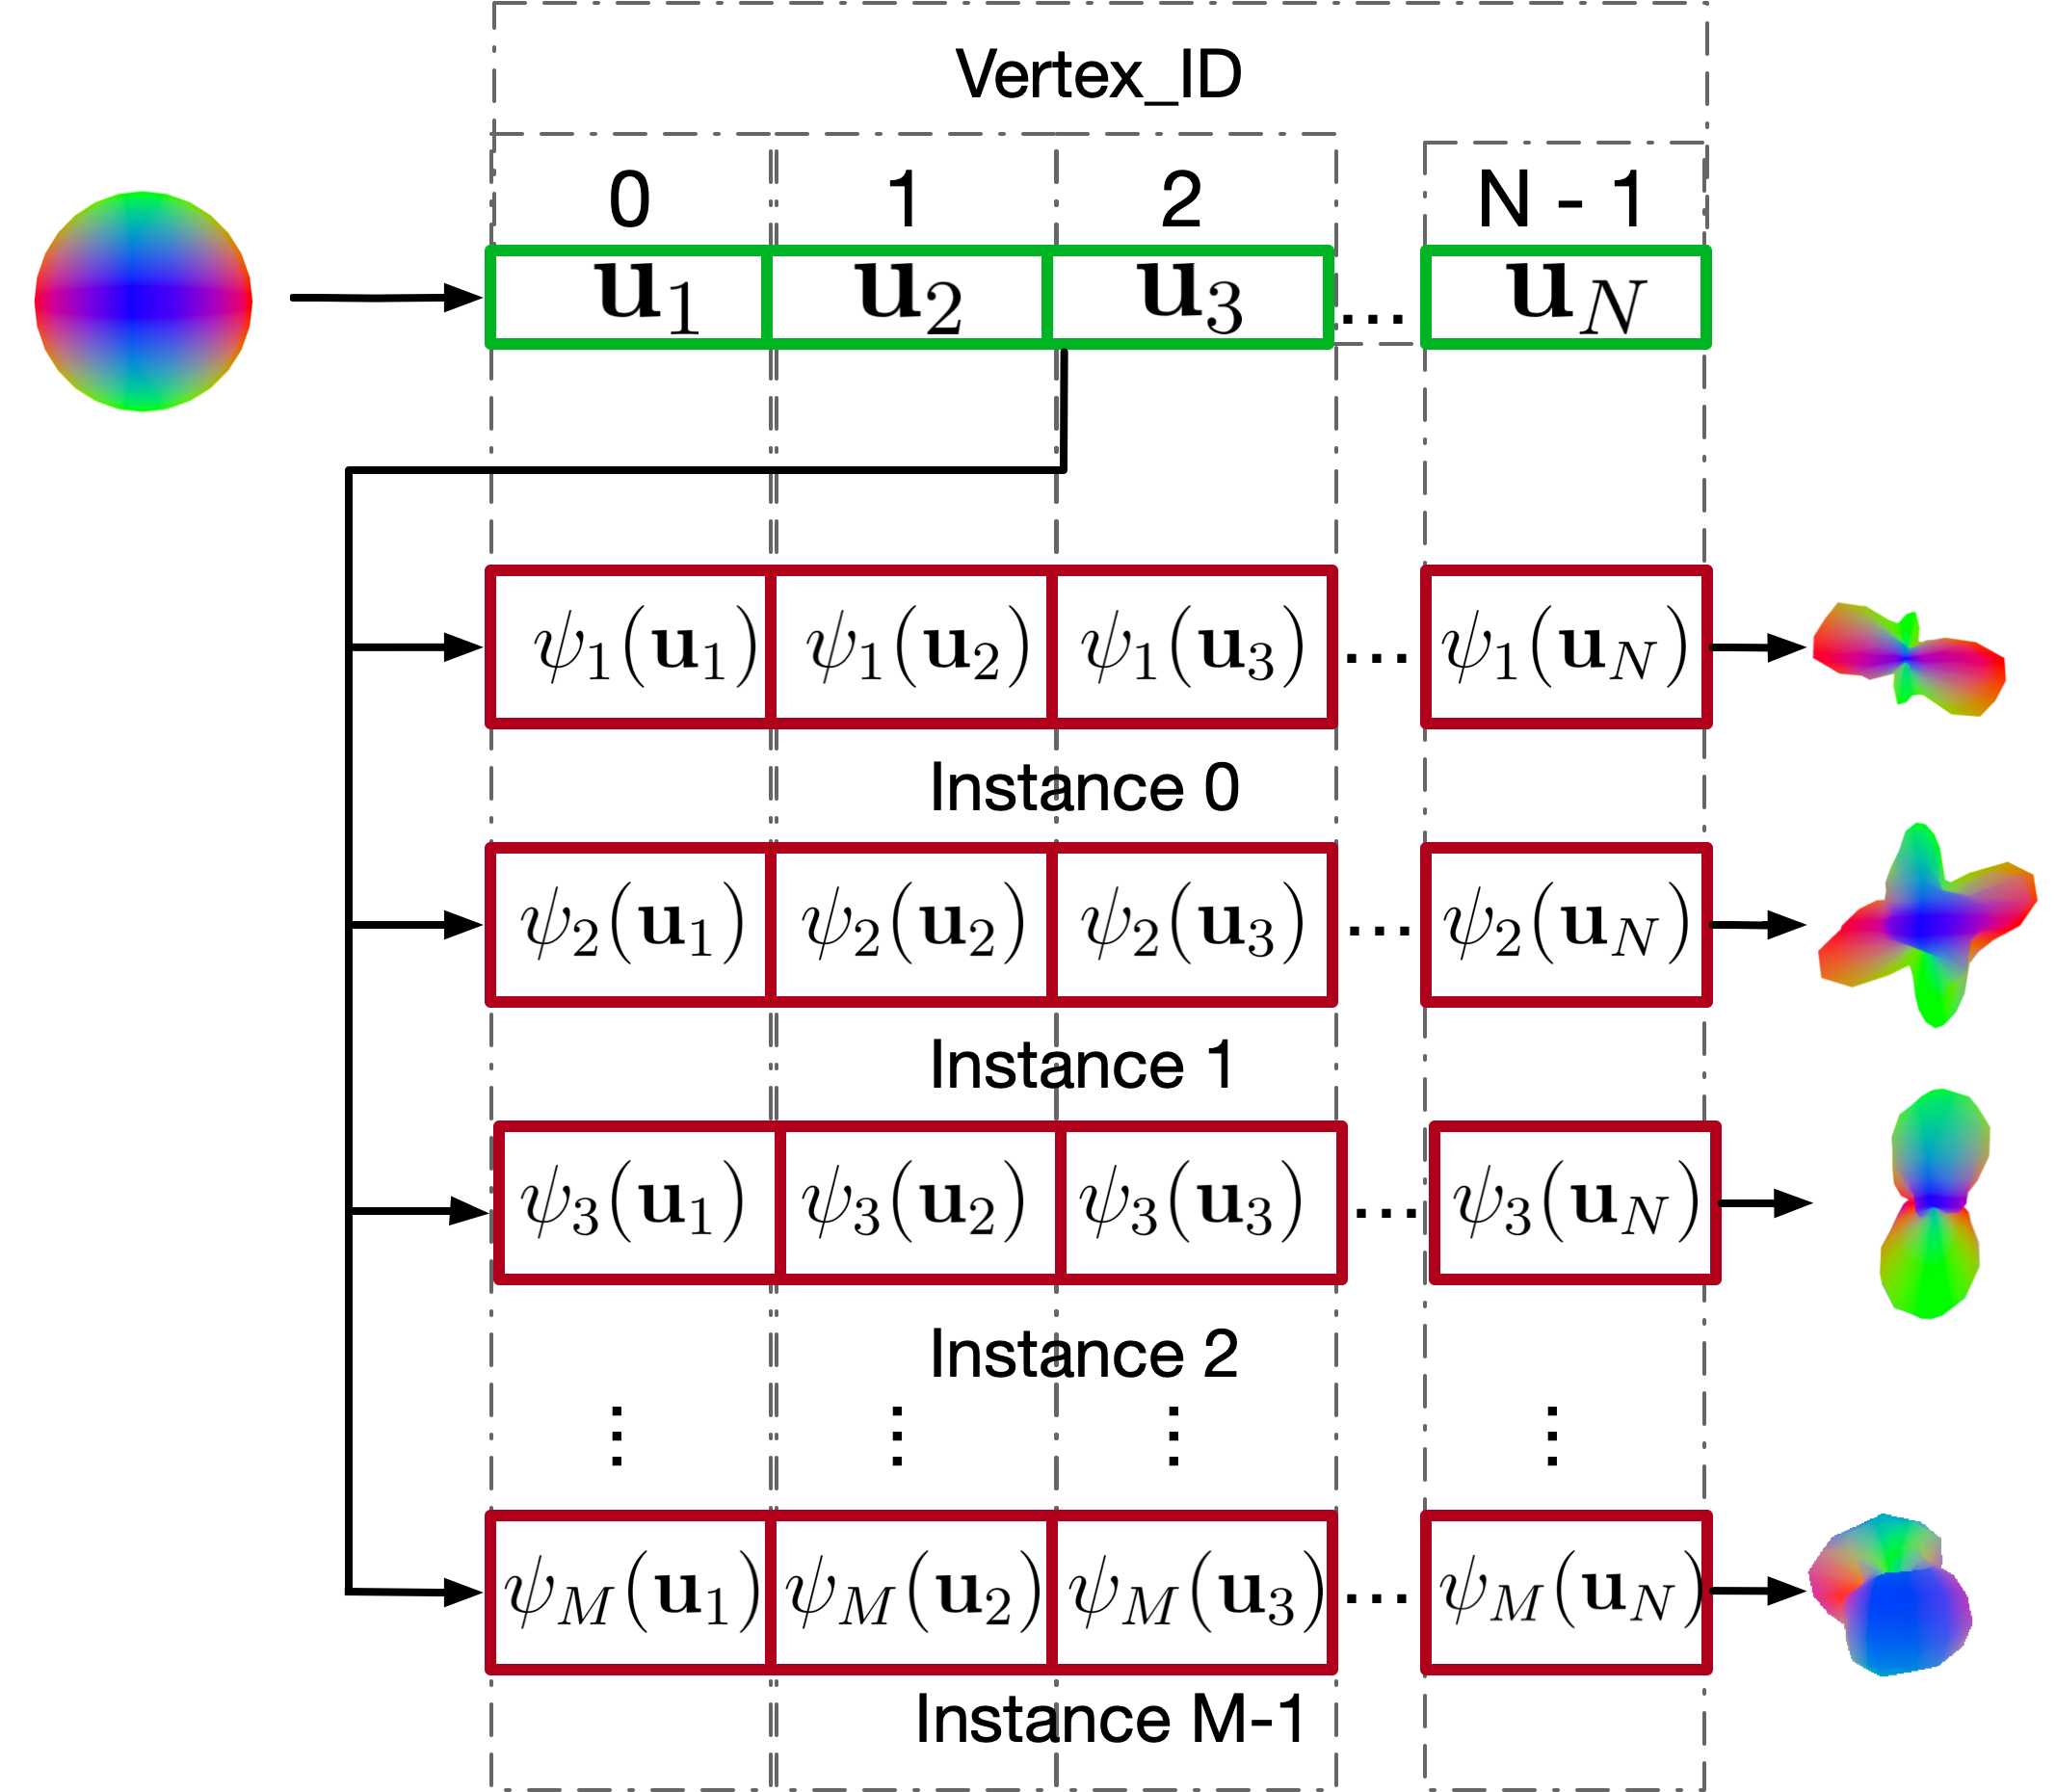
\includegraphics[width=1.0\linewidth, angle=0]{figs/rendering_scheme/GPU2Glyph.png}
    \caption{\textcolor{red}{Illustration of the data organization in the GPU of the profile matrix (red) sent as 2D-Texture. The vertices of the spherical mesh are in green. At each instance, the customization of the glyph occurs through the multiplication of the mesh vertex with its respective value, recovered in the vertex shader through its vertex index for the P glyphs to be rendered}.}
    \label{fig::GPU2glyph}
\end{figure}

%\section{Scheme Overview}
%\label{sec::scheme_overview}
%\subsection{Precomputation}
%\begin{enumerate}
%    \item Compute spherical mesh and its index buffer and send to GPU.
%\end{enumerate}
%\subsection{CPU}
%\begin{enumerate}
%    \item Compute matrix $\bm{\Psi}$ and send to GPU as a texture.
%\end{enumerate}
%\subsection{GPU}
%\subsubsection{Vertex Shader}
%\begin{enumerate}
%    \item Lookup the coefficient that customize the glyphs and multiply by the spherical vertex;
%    \item perform translation of the glyph;
%    \item do scaling and camera related transformations;
%    \item compute color as a function of the spherical mesh vertex accordingly to equation %\ref{eq::glyph_color} and send to fragment shader.
%\end{enumerate}
%\subsubsection{Fragment Shader}
%\begin{enumerate}
%    \item Set the output color as the rasterized color defined in the vertex shader.
%\end{enumerate}

%\section{Optimization}

\todo[inline]{Is it not better to put together with other part of description?}

\sout{In this section we show an adaption of the rendering scheme described in the sections \ref{sec::rendering_scheme} and \ref{sec::scheme_overview} to symmetrical ODFs and decrease the CPU-GPU data traffic by half.}

An ODF is symmetrical if $\psi(\bm{u}) = \psi(-\bm{u})$ for all $\bm{u}$ in the unit sphere. This property is present on all imaging methods for diffusion.

\textcolor{red}{Firstly, we suggest the use of a symmetrical spherical mesh, which can be, for example, any order of a sphere \todo{How? It must be explained!}generated by a tessellated icosahedron. We suggest as well that the vector containing its vertices is organized in such a way that the vector in the (2k)-th index is symmetrical to the (2k+1)-th.}

Following these recommendations, for symmetrical functions, we have $\bm{u}_{2K+2} = -\bm{u}_{2K+1}$. Then, $\bm{\Psi}$ becomes:

\begin{equation*}
\bm{\Psi} = 
\begingroup % keep the change local
\setlength\arraycolsep{2pt}
\begin{bmatrix} 
    \psi_1(\bm{u}_1) & \psi_1(-\bm{u}_1) & \cdots \psi_1(\bm{u}_{N-1}) & \psi_1(-\bm{u}_{N-1})  \\
    
     \psi_2(\bm{u}_1)& \psi_2(-\bm{u}_1) & \cdots \psi_2(\bm{u}_{N-1}) & \psi_2(-\bm{u}_{N-1}) \\

    \vdots & \vdots & \vdots & \vdots  \\
    
     \psi_P(\bm{u}_1)&\psi_P(-\bm{u}_1) & \cdots \psi_P(\bm{u}_{N-1}) & \psi_P(-\bm{u}_{N-1})
    
\end{bmatrix},
\endgroup
\end{equation*}
where each of the (2K+1)-th column is the same as 2K-th\sout{, due to the symmetry of each partial function} \textcolor{blue}{one}.

\todo{Very confusing!}We \textcolor{blue}{re}define \textcolor{blue}{Eq. \ref{eq::Psi}}, \sout{a matrix $\bm{\Psi^h}_{Px\frac{N}{2}}$ where} \textcolor{blue}{such that} $\bm{\psi^h}_{ij} = \bm{\psi}_{i(2j-1)}$. \sout{that is sent to GPU on every drawing request. Its form is stated below:}\textcolor{blue}{It assumes the form}

\begin{equation}
\label{eq::Psi_changed}
\bm{\Psi^h} = 
\begingroup % keep the change local
\setlength\arraycolsep{2pt}
\begin{bmatrix} 
    \psi_1(\bm{u}_1) & \psi_1(\bm{u}_3) & \cdots \psi_1(\bm{u}_{N-3}) & \psi_1(\bm{u}_{N-1})  \\
    
     \psi_2(\bm{u}_1)& \psi_2(\bm{u}_3) & \cdots \psi_2(\bm{u}_{N-3}) & \psi_2(\bm{u}_{N-1}) \\

    \vdots & \vdots & \vdots & \vdots  \\
    
     \psi_P(\bm{u}_1)&\psi_P(\bm{u}_3) & \cdots \psi_P(\bm{u}_{N-3}) & \psi_P(\bm{u}_{N-1})
    
\end{bmatrix}
\endgroup
\end{equation}

\sout{In}\textcolor{blue}{On} the GPU, the 2K-th and (2K+1)-th Vertex\_ID of the same instance have the same value to lookup in $\bm{\Psi}^h$, which corresponds to the K-th index of the matrix, which can be accessed accordingly in the vertex shader.



\section{Results}
Some of the results applied to a DW-MRI in the region of the corpus callosum is shown in Fig. \ref{fig::ex_glyph} and \ref{fig::ex_glyph_FAMAP} for different tesselations of the icosahedron.

\begin{figure}[t]
\centering
\captionsetup[subfloat]{farskip=0pt,nearskip=0pt}
    \subfloat[4-th order (162 vertices and 320 triangles per glyph) ]{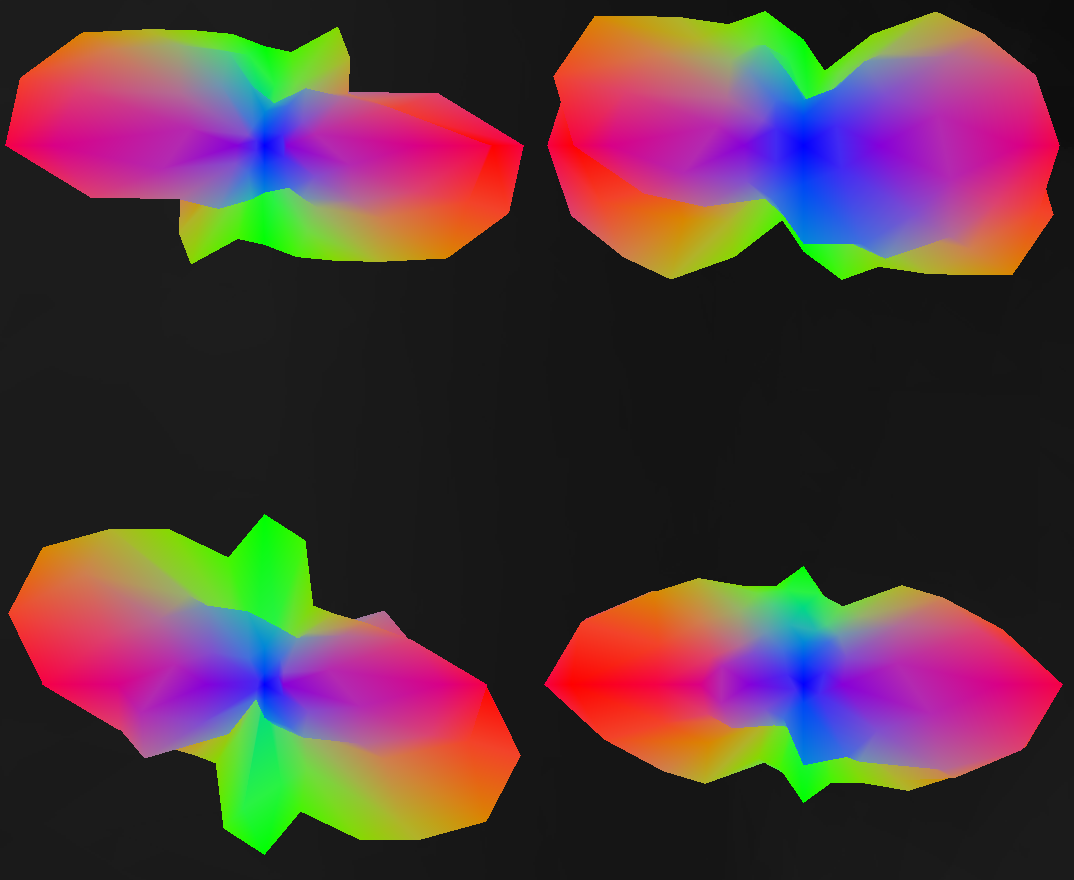
\includegraphics[width=.75\linewidth, angle=0]{figs/Results/Glyphs_4.png}}
    \\
    \subfloat[8-th order (642 vertices and 1280 triangles per glyph) ]{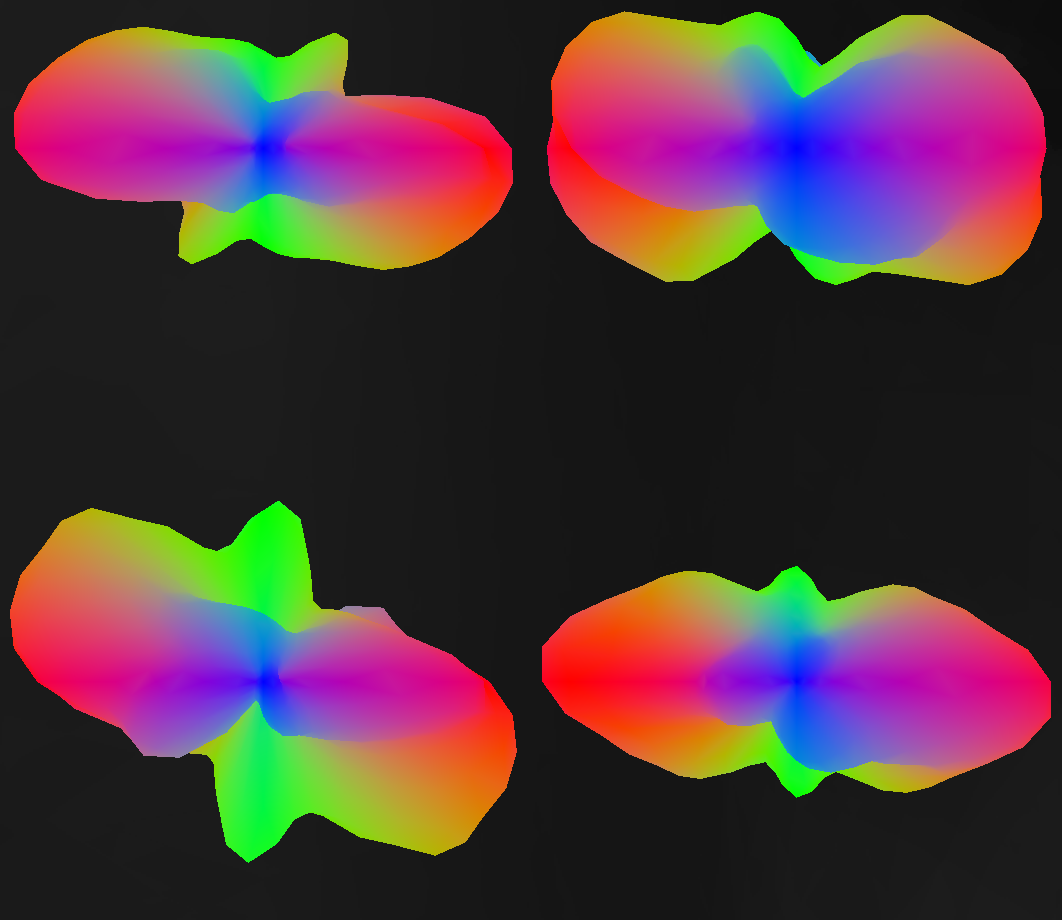
\includegraphics[width=.70\linewidth, angle=0]{figs/Results/glyphs_8.png}}
    \\
    \subfloat[16th order (2562 vertices and 5120 triangles per glyph)]{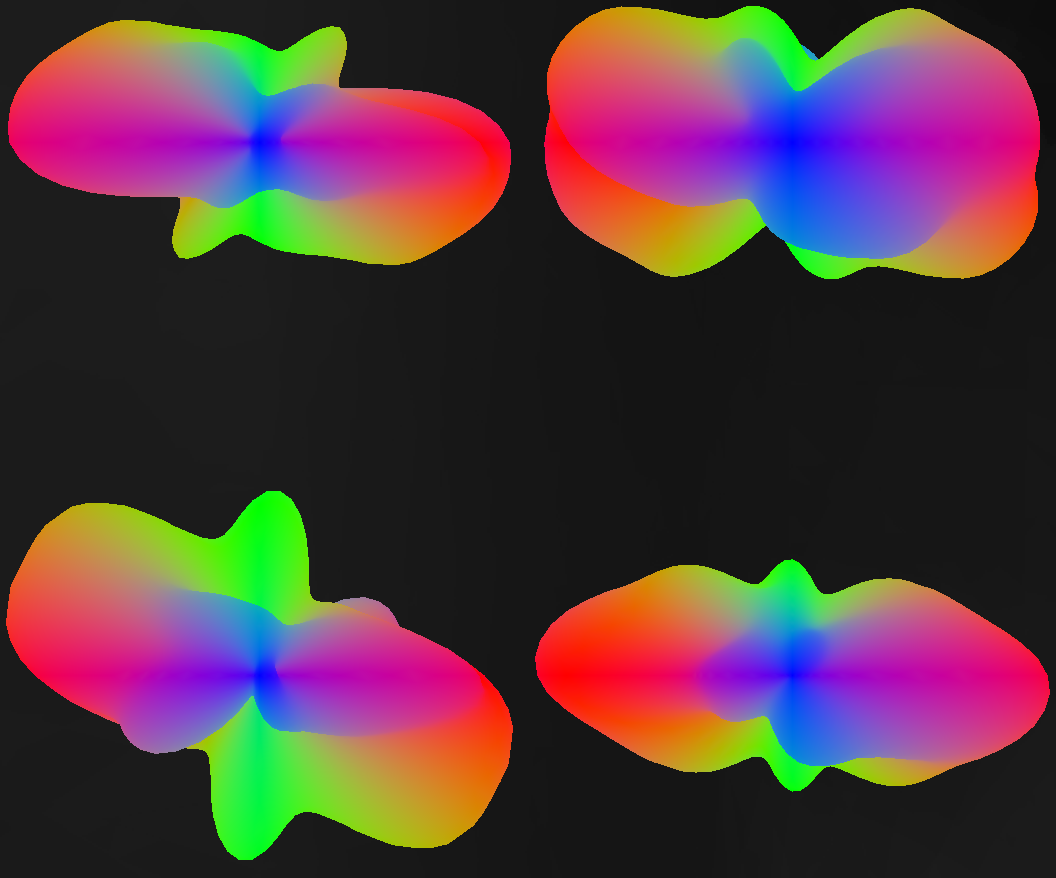
\includegraphics[width=.70\linewidth, angle=0]{figs/Results/glyphs_16.png}}
     \caption{Polygon based HARDI glyphs visualization for different orders of tessellationts of an icosahedron} %!!VER SE ISSO TA CERTO
    \label{fig::ex_glyph}
\end{figure}

\begin{figure}[htb]
    \centering
    %\rule{6cm}{3cm}
    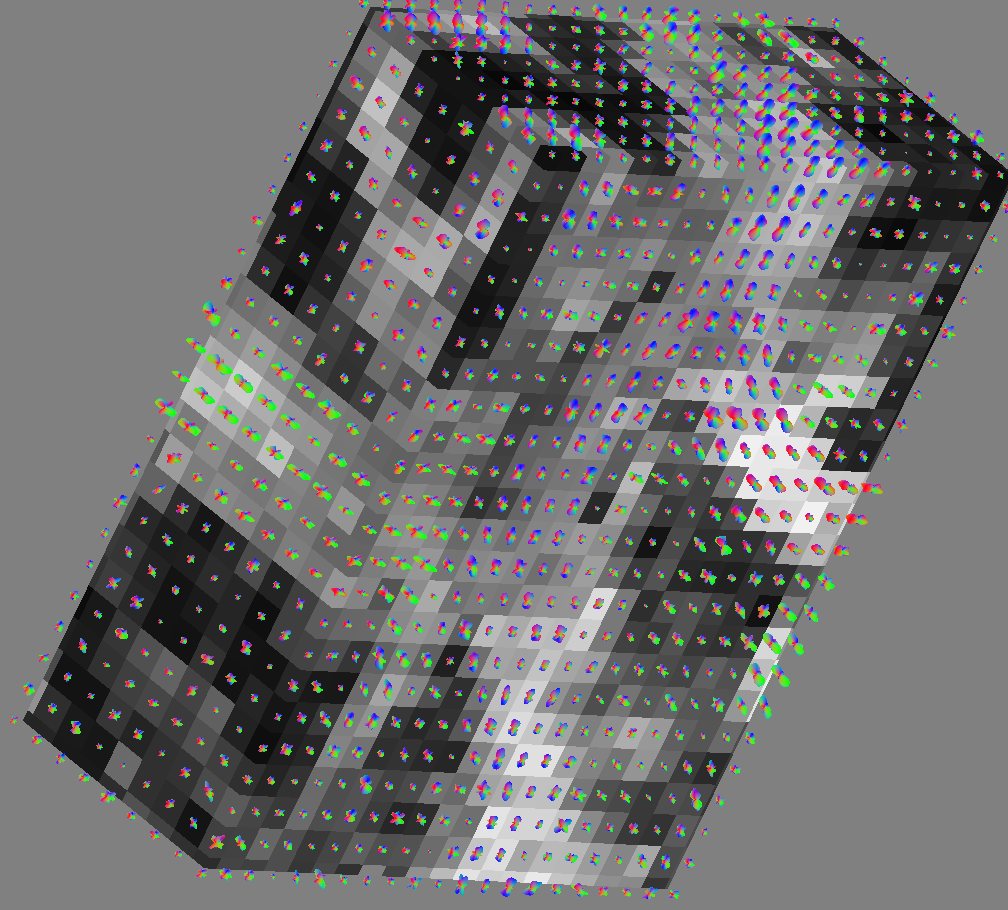
\includegraphics[width=1.00\linewidth, angle=0]{figs/Results/Glyphs_onFAMAP_2.png}
    \caption{Glyphs integrated into a DW-MRI's fractional anisotropy map. The parallelepiped shows the region where the pyramidal tract (glyphs predominantly blue) crosses the corpus callosum (predominantly red). In the middle of the left face, the predominantly green glyphs corresponds to the region of the superior longitudinal fasciculus. The spherical mesh used corresponds to an 8-th tessellated icosahedron}
    \label{fig::ex_glyph_FAMAP}
\end{figure}

\subsection{Performance}

In the tables !!refTable follows the benchmark of the rendering scheme. The benchmark consists of the time of copying pre processed data to send to the GPU and the GPU processing and drawing time. If the ODFs are stored as coefficients of spherical harmonics, it needs a step of sampling over an spherical mesh.

\subsection{\textcolor{blue}{An Application}}

\todo[inline]{To assess the fiber orientations locally?}

\section{Conclusions}

In this work we presented a rendering scheme to render multiple ODFs at interactive rates. We used polygons approach and suggested procedures to decrease the data traffic CPU-GPU in drawing requests.

We also suggested a optimization procedure to decrease the data computation and traffic between CPU by half on symmetrical ODFs.

The rendering scheme proved to be fast enough to render hundreds of objects, which meshes are fine sufficiently to make the surfaces appear smooth.

That scheme can be integrated with other DW-MRI and MRI visualization schemes. It can be a very useful tool to render each ODF's glyph on its respective voxel in the scene.







%\section{Page size}
%Permission to make digital or hard copies of all or part of this work for personal or classroom use is granted without fee provided that copies are not made or distributed for profit or commercial advantage and that copies bear this notice and the full citation on the first page. To copy otherwise, or republish, to post on servers or to redistribute to lists, requires prior specific permission and/or a fee. 

%All material on all pages should fit within a rectangle of 16 x 23.7 cm (6.3"x 9.33"), centered on the page horizontally, beginning 2.5 cm (1") from the top of the page and ending with 3,5 cm (1.4") from the bottom.  The right and left margins should be 2.5 cm (1"). The text should be in two 7.6 cm (3") columns with a 0.8 cm (0.3") gutter. 

%\section{Typeset text}
%\subsection*{Normal or Body Text}
%Please use a 10-point Times Roman font, or other Roman font with serifs, as close as possible in appearance to Times Roman in which these guidelines have been set. The goal is to have a 10-point text, as you see here. Please use sans-serif or non-proportional fonts only for special purposes, such as distinguishing source code text. If Times Roman is not available, try the font named Computer Modern Roman. On a Macintosh, use the font named Times.  Right margins should be justified, not ragged.

%\subsection*{Title and Authors}
%The title (Helvetica 18-point bold), authors' names (Helvetica 10-point) and affiliations (Helvetica 10 point) run across the full width of the page -- one column wide. We also recommend e-mail address (Helvetica 10 point). See the top of this page for three addresses. If only one address is needed, center all address text. For two addresses, use two centered tabs, and so on. For more than three authors, you may have to improvise.\footnote{If necessary, you may place some address information in a footnote, or in a named section at the end of your paper, but margins must remain empty.} 

%\subsection*{First Page Copyright Notice}
%Please include 3.8 cm (1.5") text box with the text shown at the bottom of the left column of the first page with the copyright notice.

%\subsection*{Others Pages}
%Others pages start at the top of the page (margin 2.5 cm) and continue in double-column format.  The two columns on the last even page should be as close to equal length as possible. 

%{\bfseries Total length of a paper is max. 8 pages.}

%Footnotes should be Times New Roman 9-point, and justified to the full width of the column.

%Please, use the standard Journal of WSCG format for references -- that is, a numbered list at the end of the article, ordered alphabetically by first author, and referenced by a name in brackets \cite{con00a}. See the examples of citations at the end of this document. Within this template file, use the style named references for the text of your citation.

%The references are also in 9 pt., but that section (see Section \ref{references}) is ragged right. References should be published materials accessible to the public. Internal technical reports may be cited only if they are easily accessible (i.e. you can give the address to obtain the report within your citation) and may be obtained by any reader. Proprietary information may not be cited. Private communications should be acknowledged, not referenced, e.g. "[Adam, personal communication]").

%\subsection*{Page Numbering, Headers and Footers}
%Do not include headers, footers or page numbers in your submission. These will be added when the publications are assembled.

%\begin{figure}[htb]
%    \centering
%    \rule{6cm}{3cm}
%    \caption{Insert caption to place caption below figure.}
%    \label{fig:box}
%\end{figure}

%\begin{table}[htb]
%	\centering
%	\begin{tabular}{|l|l|l|l|}
%	\hline
%	Graphics & Top & In-between & Bottom \\
%	\hline
%	Tables & End & Last & First \\
%	\hline
%	Figures & Good & Similar & Very well \\
%	\hline
%	\end{tabular}
%	\caption{Table captions should be placed below the table}
%\end{table}

%\section{Figures/Captions}
%Place Tables/Figures/Images in text as close to the reference as possible (see Fig.\ref{fig:box}). It may extend across both columns to a maximum width of 16 cm (6.3"). Captions should be Times New Roman 10-points.  They should be numbered (e.g., "Table 1" or "Figure 2"), please note that the word for Table and Figure are spelled out. Figure's and Table's captions should be centered beneath the image, picture or a table.

%\section{Sections}
%The heading of a section should be in Times New Roman 12-point bold in all-capitals flush left with an additional 6-points of white space above the section head.  Sections and subsequent sub- sections should be numbered and flush left. For a section head and a subsection head together (such as Section 3 and Subsection 3.1), use no additional space above the subsection head.

%\subsection{Subsections}
%The heading of subsections should be in Times New Roman 12-point bold with only the initial letters capitalized. (Note: For subsections and subsubsections, a word like the or a is not capitalized unless it is the first word of the header.)

%\subsubsection{Subsubsections}
%The heading for subsubsections should be in Times New Roman 11-point italic with initial letters capitalized and 6-points of white space above the subsubsection head.

%\section{Acknowledgments}
%Our thanks to ACM SIGCHI and SIGGRAPH for allowing us to modify templates they had developed.

%-------------------------------------------------------------------------
% example of algorithm typesetting
% to allow this, uncomment line 
% \RequirePackage[noend]{myalgorithm}
% in the wscg.sty file
% and download that package from Gabriel Zachmann's page http://zach.in.tu-clausthal.de/latex/
%
%
%\begin{algorithm}
%\hrule
%  \centering
%\begin{algorithmic}
%    \STMT $d_{l,r} = f_B(P_1), f_B(P_n)$
%    \WHILE{ $|d_l| > \epsilon $ and $|d_r| > \epsilon $ and $l<r$}
%        \STMT $d_x = f_B(P_x)$
%        \IF{ $d_x < 0$ }
%            \STMT $l, r = x, r$
%        \ELSE
%            \STMT $l, r = l, x$
%        \ENDIF
%    \ENDWHILE
%\end{algorithmic}
%\hrule
%\caption{Example of some pseudo-code}
%\label{fg:code}
%\end{algorithm}


%-------------------------------------------------------------------------

\printbibliography
%\begin{thebibliography}{99}
%\label{references}
%\label{references}
%\bibitem[And01a]{and01a} Anderson, R.E. Social %impacts of computing: Codes of professional %ethics. Social Science, pp.453-469, 2001.
%\bibitem[Con00a]{con00a} Conger., S., and Loch, %K.D. (eds.). Ethics and computer use. Com.of ACM %38, No.12, 2000.
%\bibitem[Con00b]{con00b} Mackay, W.E. Ethics, lies %and videotape, in Conf.proc. CHI'00, Denver CO, %ACM Press, pp.138-145, 2000.
%\bibitem[Jou01a]{jou01a} Journal of WSCG \& WSCG %templates: http://wscg.zcu.cz/jwscg/template.doc %(MSWord)
%http://wscg.zcu.cz/jwscg/template.pdf (PDF)
%\end{thebibliography}
%{\bfseries


%Last page should be fully used by text, figures etc. Do not leave empty space, please. 
%Do not lock the PDF -- additional text and info will be inserted, i.e. ISSN/ISBN etc. 
%}
\end{document}